\section{Auswertung}
\label{sec:auswertung}

Die Auswertung der aufgenommen Messdaten sei in drei Abschnitte unterteilt.

\subsection{Mittlere freie Weglänge und Dampfdruck}

Zunächst sollen der Dampfdruck sowie die mittlere freie Weglänge zu den verwendeten Temperaturen bestimmt werden.
Mithilfe von \eqref{eq:mittfreiweg} und \eqref{eq:dampfdruck} ergeben sich die in \autoref{tab:dampfd_freiweg} dargestellten Werte.

\begin{table}[H]
    \centering
    \caption{Dampfdruck $p_\text{sät}$, mittlere freie Weglänge $\bar{w}$ sowie der Faktor $\frac{a}{\bar{w}}$ zu unterschiedlichen Temperaturen $T$.}
    \label{tab:dampfd_freiweg}
    \begin{tabular}{S[table-format = 3.1] S[table-format = 2.4] S[table-format = 1.7] S[table-format = 4.2]}
      \toprule
      {$T \mathbin{/} \unit{\celsius}$} & {$p_\text{sät} \mathbin{/} \unit{\milli\bar}$} & {$\bar{w} \mathbin{/} \unit{\centi\meter}$} & {$\frac{a}{\bar{w}}$} \\
      \midrule
       25.7         &            0.0056          &           0.5180465           &              1.93        \\
      142.0         &            3.5260          &           0.0008225           &           1215.85        \\
      173.5         &           11.1450          &           0.0002602           &           3843.09        \\
      191.2         &           20.3901          &           0.0001422           &           7031.06        \\
      \bottomrule
    \end{tabular}
\end{table}

Neben der mittleren freien Weglänge und dem Sättigungsdampfdruck ist in \autoref{tab:dampfd_freiweg} auch der Faktor $\frac{a}{\bar{w}}$ aufgetragen, wobei $a = 1 \,\unit{\centi\meter}$ als Abstand zwischen Kathode
und Beschleunigerelektrode angenommen wird.


\subsection{Bestimmung der integralen Energieverteilung}

Die mit dem XY-Schreiber aufgenommenen Kurven sind in \autoref{fig:grapha} zu erkennen, wobei die Messung bei $25,7 \,\unit{\celsius}$ die Messung bei Raumtemperatur darstellt.

\begin{figure}[H]
    \centering
    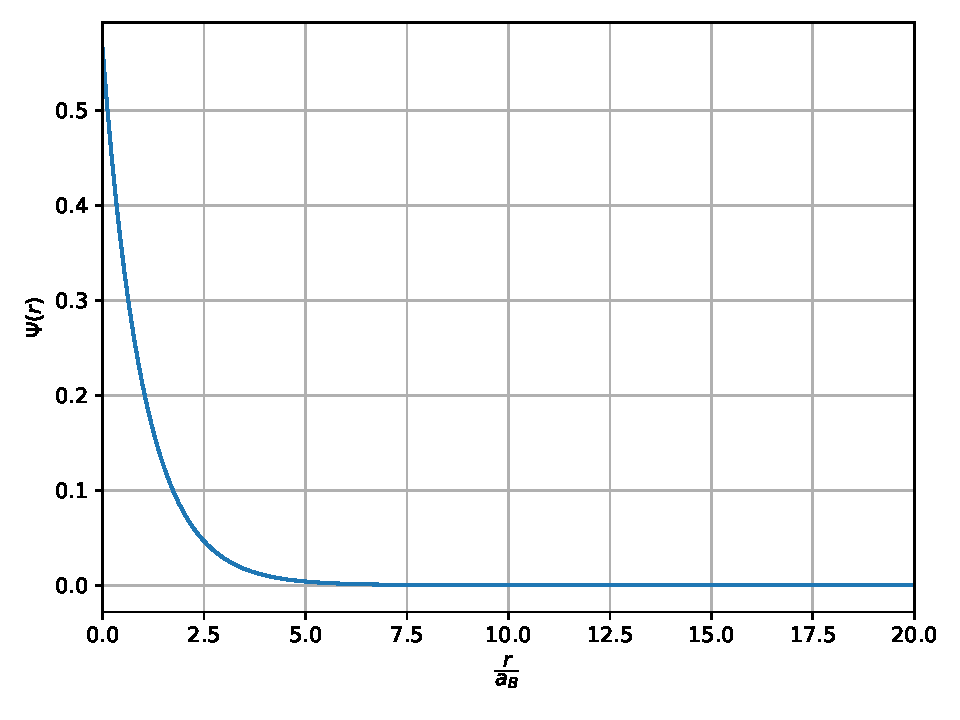
\includegraphics{build/Graph_a.pdf}
    \caption{Auffängerstrom $I_\text{A}$ in Abhängigkeit von $U_\text{A}$ bei $25,7 \,\unit{\celsius}$ bzw. $142 \,\unit{\celsius}$.}
    \label{fig:grapha}
\end{figure}

Wird nun die Bremsspannung $U_\text{A}$ gegen die Differenz $I_\text{A}(U_\text{A}+ \Delta U_\text{A}) - I_\text{A}(U_\text{A})$ geplottet, ergeben sich die in \autoref{fig:graphb} zu erkennenden Graphen.

\begin{figure}[H]
    \centering
    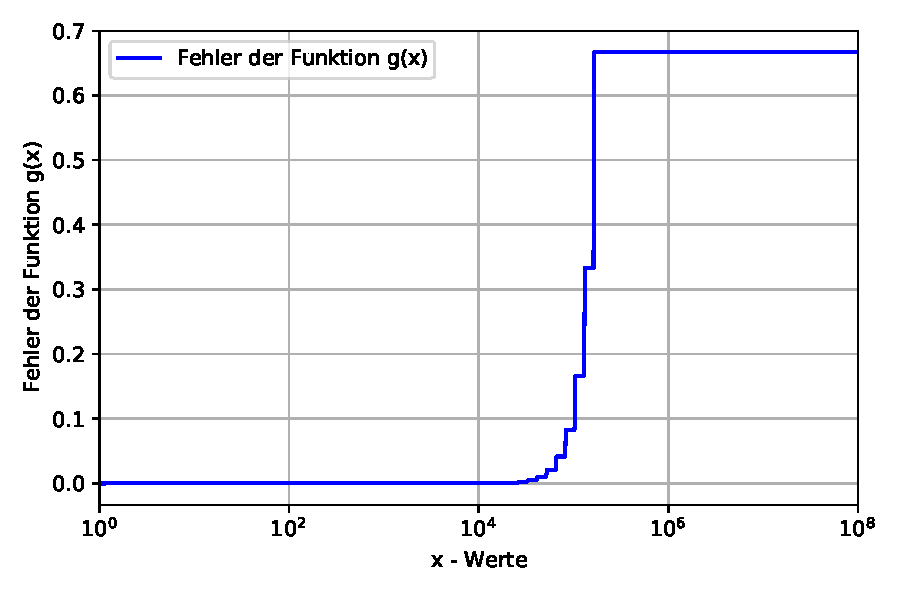
\includegraphics{build/Graph_b.pdf}
    \caption{Differenz $I_\text{A}(U_\text{A}+ \Delta U_\text{A}) - I_\text{A}(U_\text{A})$ in Abhängigkeit der Spannung $U_\text{A}$.}
    \label{fig:graphb}
\end{figure}

Die Verbindungen zwischen den Punkten dienen dabei nur der besseren Viualisierung und besitzen keinerlei physikalische Relevanz.
Das bei der blauen Kurve erkennbare Minimum entspricht der effektiven Beschleunigungsspannung $U_{\text{B},\text{eff}}$ bei $U_{\text{B},\text{eff}} = 8 \,\unit{\volt}$, wie sie in \eqref{eq:Ueff} zum Einsatz kommt.
Zusammen mit der eingestellten Beschleunigungsspannung von $U_\text{B} = 11 \,\unit{\volt}$ lässt sich das Kontaktpotential $K$ zu
\begin{equation*}
    K = \frac{1}{\text{e}_0} (\Phi_\text{B} - \Phi_\text{G}) = U_\text{B} - U_{\text{B},\text{eff}} = 3 \,\unit{\volt} %% passt das so?
\end{equation*}
bestimmen.


\subsection{Auswertung der Franck-Hertz-Kurven}

Mithilfe des XY-Schreibers wurden die in \autoref{fig:graphc} und \autoref{fig:graphd} dargestellten Kurven aufgenommen.

\begin{figure}[H]
    \centering
    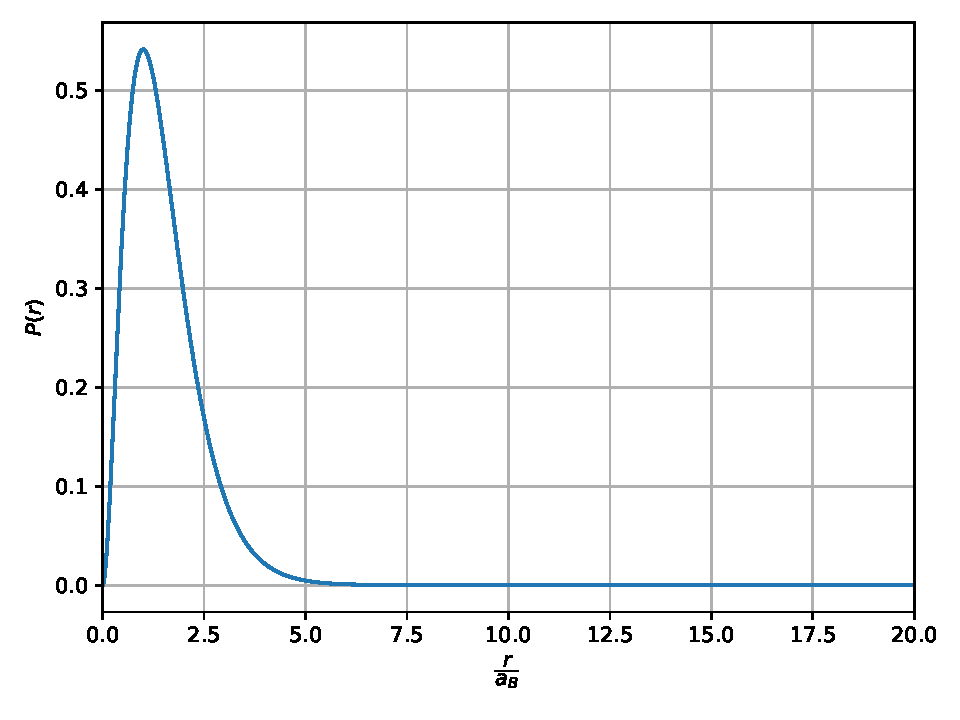
\includegraphics{build/Graph_c.pdf}
    \caption{Franck-Hertz-Kurve bei $173,5 \,\unit{\celsius}$.}
    \label{fig:graphc}
\end{figure}

\begin{figure}[H]
  \centering
  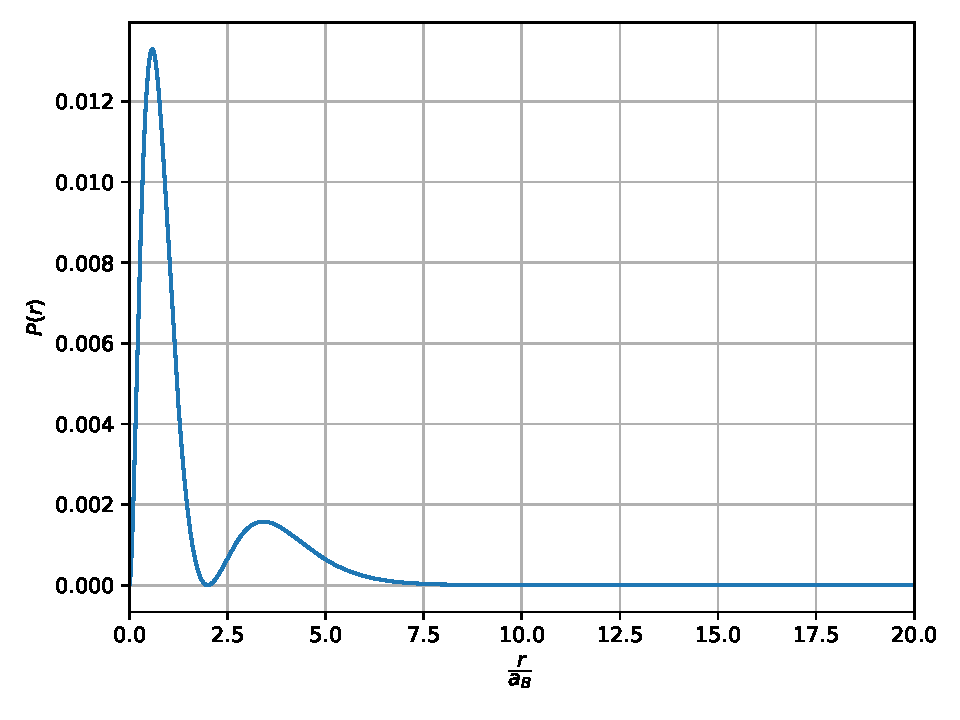
\includegraphics{build/Graph_d.pdf}
  \caption{Franck-Hertz-Kurve bei $191,2 \,\unit{\celsius}$.}
  \label{fig:graphd}
\end{figure}

Die Positionen des $i$-ten, in \autoref{fig:graphc} rot markierten Maximums sind in \autoref{tab:iiplus1} dargestellt.
Das erste Maximum beschreibt dabei das erste erkennbare Maximum, auch wenn von mindestens einem weiteren, nicht sichtbaren Maximum ausgegangen werden kann.

\begin{table}[H]
    \centering
    \caption{Abstand des $i$-ten Maximums bei $173,5 \,\unit{\celsius}$ bzw. $191,2 \,\unit{\celsius}$ vom Nullpunkt.}
    \label{tab:iiplus1}
    \begin{tabular}{S[table-format = 1.1] S[table-format = 2.1] S[table-format = 2.2]}
      \toprule
      {$i$-tes Maximum} & {$T = 173,5 \,\unit{\celsius}$} & {$T = 191,2 \,\unit{\celsius}$}\\
      \midrule
       %%%%%%%%%%%%% Hier könnten Ihre Werte stehen
        {1}               &           {16.5}           &           {13.5}            \\
        {2}               &           {22.8}           &           {19.5}            \\
        {3}               &           {30.6}           &           {25.25}           \\
        {4}               &           {37.6}           &           {31.25}           \\
        {5}               &           {46.6}           &           {37.5}            \\
        {6}               &           {-}              &           {43.5}           \\
        {7}               &           {-}              &           {49.75}          \\
        %%%%%%%%%%%%%%%%%%%%%%%
      \bottomrule
    \end{tabular}
\end{table}

Von Bedeutung sind hier aber insbesondere die in \autoref{tab:messung2diffs} dargestellten Abstände zwischen dem $i$-ten und $i + 1$-ten Maximum.

\begin{table}[H]
    \centering
    \caption{Differenz zwischen $i$-tem und $i + 1$-tem Maximum bei $173,5 \,\unit{\celsius}$ bzw. $191,2 \,\unit{\celsius}$.}
    \label{tab:messung2diffs}
    \begin{tabular}{S[table-format = 1.1] S[table-format = 2.3] S[table-format = 2.3]}
      \toprule
      {} & {$T = 173,5 \,\unit{\celsius}$} & {$T = 191,2 \,\unit{\celsius}$}\\
      \midrule
       %%%%%%%%%%%%% Hier könnten Ihre Werte stehen
        {1-2}               &           {6,3}           &           {6,0}              \\
        {2-3}               &           {7,8}           &           {5,75}           \\
        {3-4}               &           {7,0}           &           {6,0}            \\
        {4-5}               &           {9,0}           &           {6,25}           \\
        {5-6}               &           {-}             &           {6,0}            \\
        {6-7}               &           {-}             &           {6.25}           \\
        %%%%%%%%%%%%%%%%%%%%%%%
      \bottomrule
    \end{tabular}
\end{table}

Die berechneten Differenzen lassen sich zu den in \autoref{tab:mittelwertis} aufgetragenen Werten mitteln, die Energie ist dabei durch
$E = q \Delta U$ gegeben.

\begin{table}[H]
    \centering
    \caption{Mittelwerte und Abweichungen der Maximadifferenzen bei $173,5 \,\unit{\celsius}$ bzw. $191,2 \,\unit{\celsius}$.}
    \label{tab:mittelwertis}
    \begin{tabular}{S[table-format = 1.1] S[table-format = 2.3] S[table-format = 2.3]}
      \toprule
      {} & {$\Delta U \mathbin{/} \unit{\volt}$} & {$E \mathbin{/} \unit{\eV}$}\\
      \midrule
       %%%%%%%%%%%%% Hier könnten Ihre Werte stehen
       {$T = 173,5 \,\unit{\celsius}$}      &     {$  7,525 \pm \, 1,003$}   & {$  7,525 \pm \, 1,003$} \\
       {$T = 191,2 \,\unit{\celsius}$}      & 	  {$ 6,042 \pm 0,172 $}       & {$6,042 \pm 0,172      $} \\
      \bottomrule
    \end{tabular}
\end{table}

So lassen sich nun aus \eqref{eq:emittwellläng} die Wellenlänge der beim Energieübergang emittierten Lichtquanten bestimmen.
Es ergeben sich die in \autoref{tab:wellenläng} niedergeschriebenen Werte.

\begin{table}[H]
    \centering
    \caption{Emittierte Wellenlängen $\lambda$ bei $173,5 \,\unit{\celsius}$ bzw. $191,2 \,\unit{\celsius}$.}
    \label{tab:wellenläng}
    \begin{tabular}{S S[table-format = 2.3] S[table-format = 2.3]}
      \toprule
      {}      &     {Bei $T = 173,5 \,\unit{\celsius}$} & {Bei $T = 191,2 \,\unit{\celsius}$}\\
      \midrule
       %%%%%%%%%%%%% Hier könnten Ihre Werte stehen
         {$\lambda$}      &       {$\left( 165 \pm 22 \right)\, \unit{\nano\meter}$}      &     {$\left( 206 \pm 6 \right) \, \unit{\nano\meter}$}           \\
        %%%%%%%%%%%%%%%%%%%%%%%
      \bottomrule
    \end{tabular}
\end{table}